%%=============================================================================
%% Methodologie
%%=============================================================================

\chapter{\IfLanguageName{dutch}{Methodologie}{Methodology}}%
\label{ch:methodologie}
\section{Dataverwerking}
\subsection{Technologieën voor databases}
In het eerste deel van deze bachelorproef wordt er een literatuurstudie uitgevoerd over de verschillende technologieën die we gebruiken om onze data op te slaan en te verwerken.
Hier hebben we de werking en efficiëntie van CosmosDB onderzocht. Daarnaast hebben we ook gekeken naar de werking van Gremlin API en hoe we deze kunnen gebruiken om een grafiekmodel op te zetten.
De data die we ontvangen is vrij ingewikkelde data. Dit is namelijk een boomstructuur uit SAP die we via een JSON bestand hebben ontvangen.
Het moeilijkste aan deze data is de interpretatie van de verschillende sleutel-waarde paren en de hierarchie die niet volledig klopt, waardoor de juiste verdeling tussen afdeling of machine moeilijker was. 
Elke sleutel heeft een specifieke betekenis en waarde die we moeten vertalen naar een leesbare vorm voor het grafiekmodel.
Na het verwerken, begrijpen en opschonen van de data, hebben we deze data omgezet naar JSON-LD formaat met de GS1-standaarden.
Vanaf dit moment is de data klaar om te worden ingeladen in CosmosDB.\@
Door gebruik te maken van Python en Javascript kunnen we grote delen van het proces automatiseren, waardoor we sneller en efficiënter kunnen werken.

\section{Proof of concept}
\subsection{Opzetten van een grafiekmodel}
In het tweede deel van deze bachelorproef wordt er een proof of concept opgesteld van het grafiekmodel waarbij we de SAP data van ArcelorMittal Gent zullen gebruiken.
Zoals eerder vermeld hebben we de van JSON data omgezet naar GS1-standaarden in een JSON-LD bestand. Dit bestand dat opgemaakt is met schema.org en GS1 EPCIS-events wordt ingeladen in CosmosDB via NodeJS en Gremlin API.\@
Daardoor ontstaat een grafiekmodel waarin we de data kunnen visualiseren en analyseren door de relaties tussen de verschillende producten en processen.
Dit grafiekmodel kan gevisualiseerd worden met behulp van Graph Explorer die ingebouwd is in Azure CosmosDB of andere visualisatie tools. 
In figuur~\ref{fig:workflow} is een voorbeeld te zien van de werking van de chatbot.
In het eerste deel van de figuur is te zien wat er moet gebeuren met de data indien deze geen JSON-LD formaat heeft.
In het tweede deel wordt weergegeven hoe de chatbot van een vraag tot een antwoord gaat.

\begin{figure}[H]
    \centering
    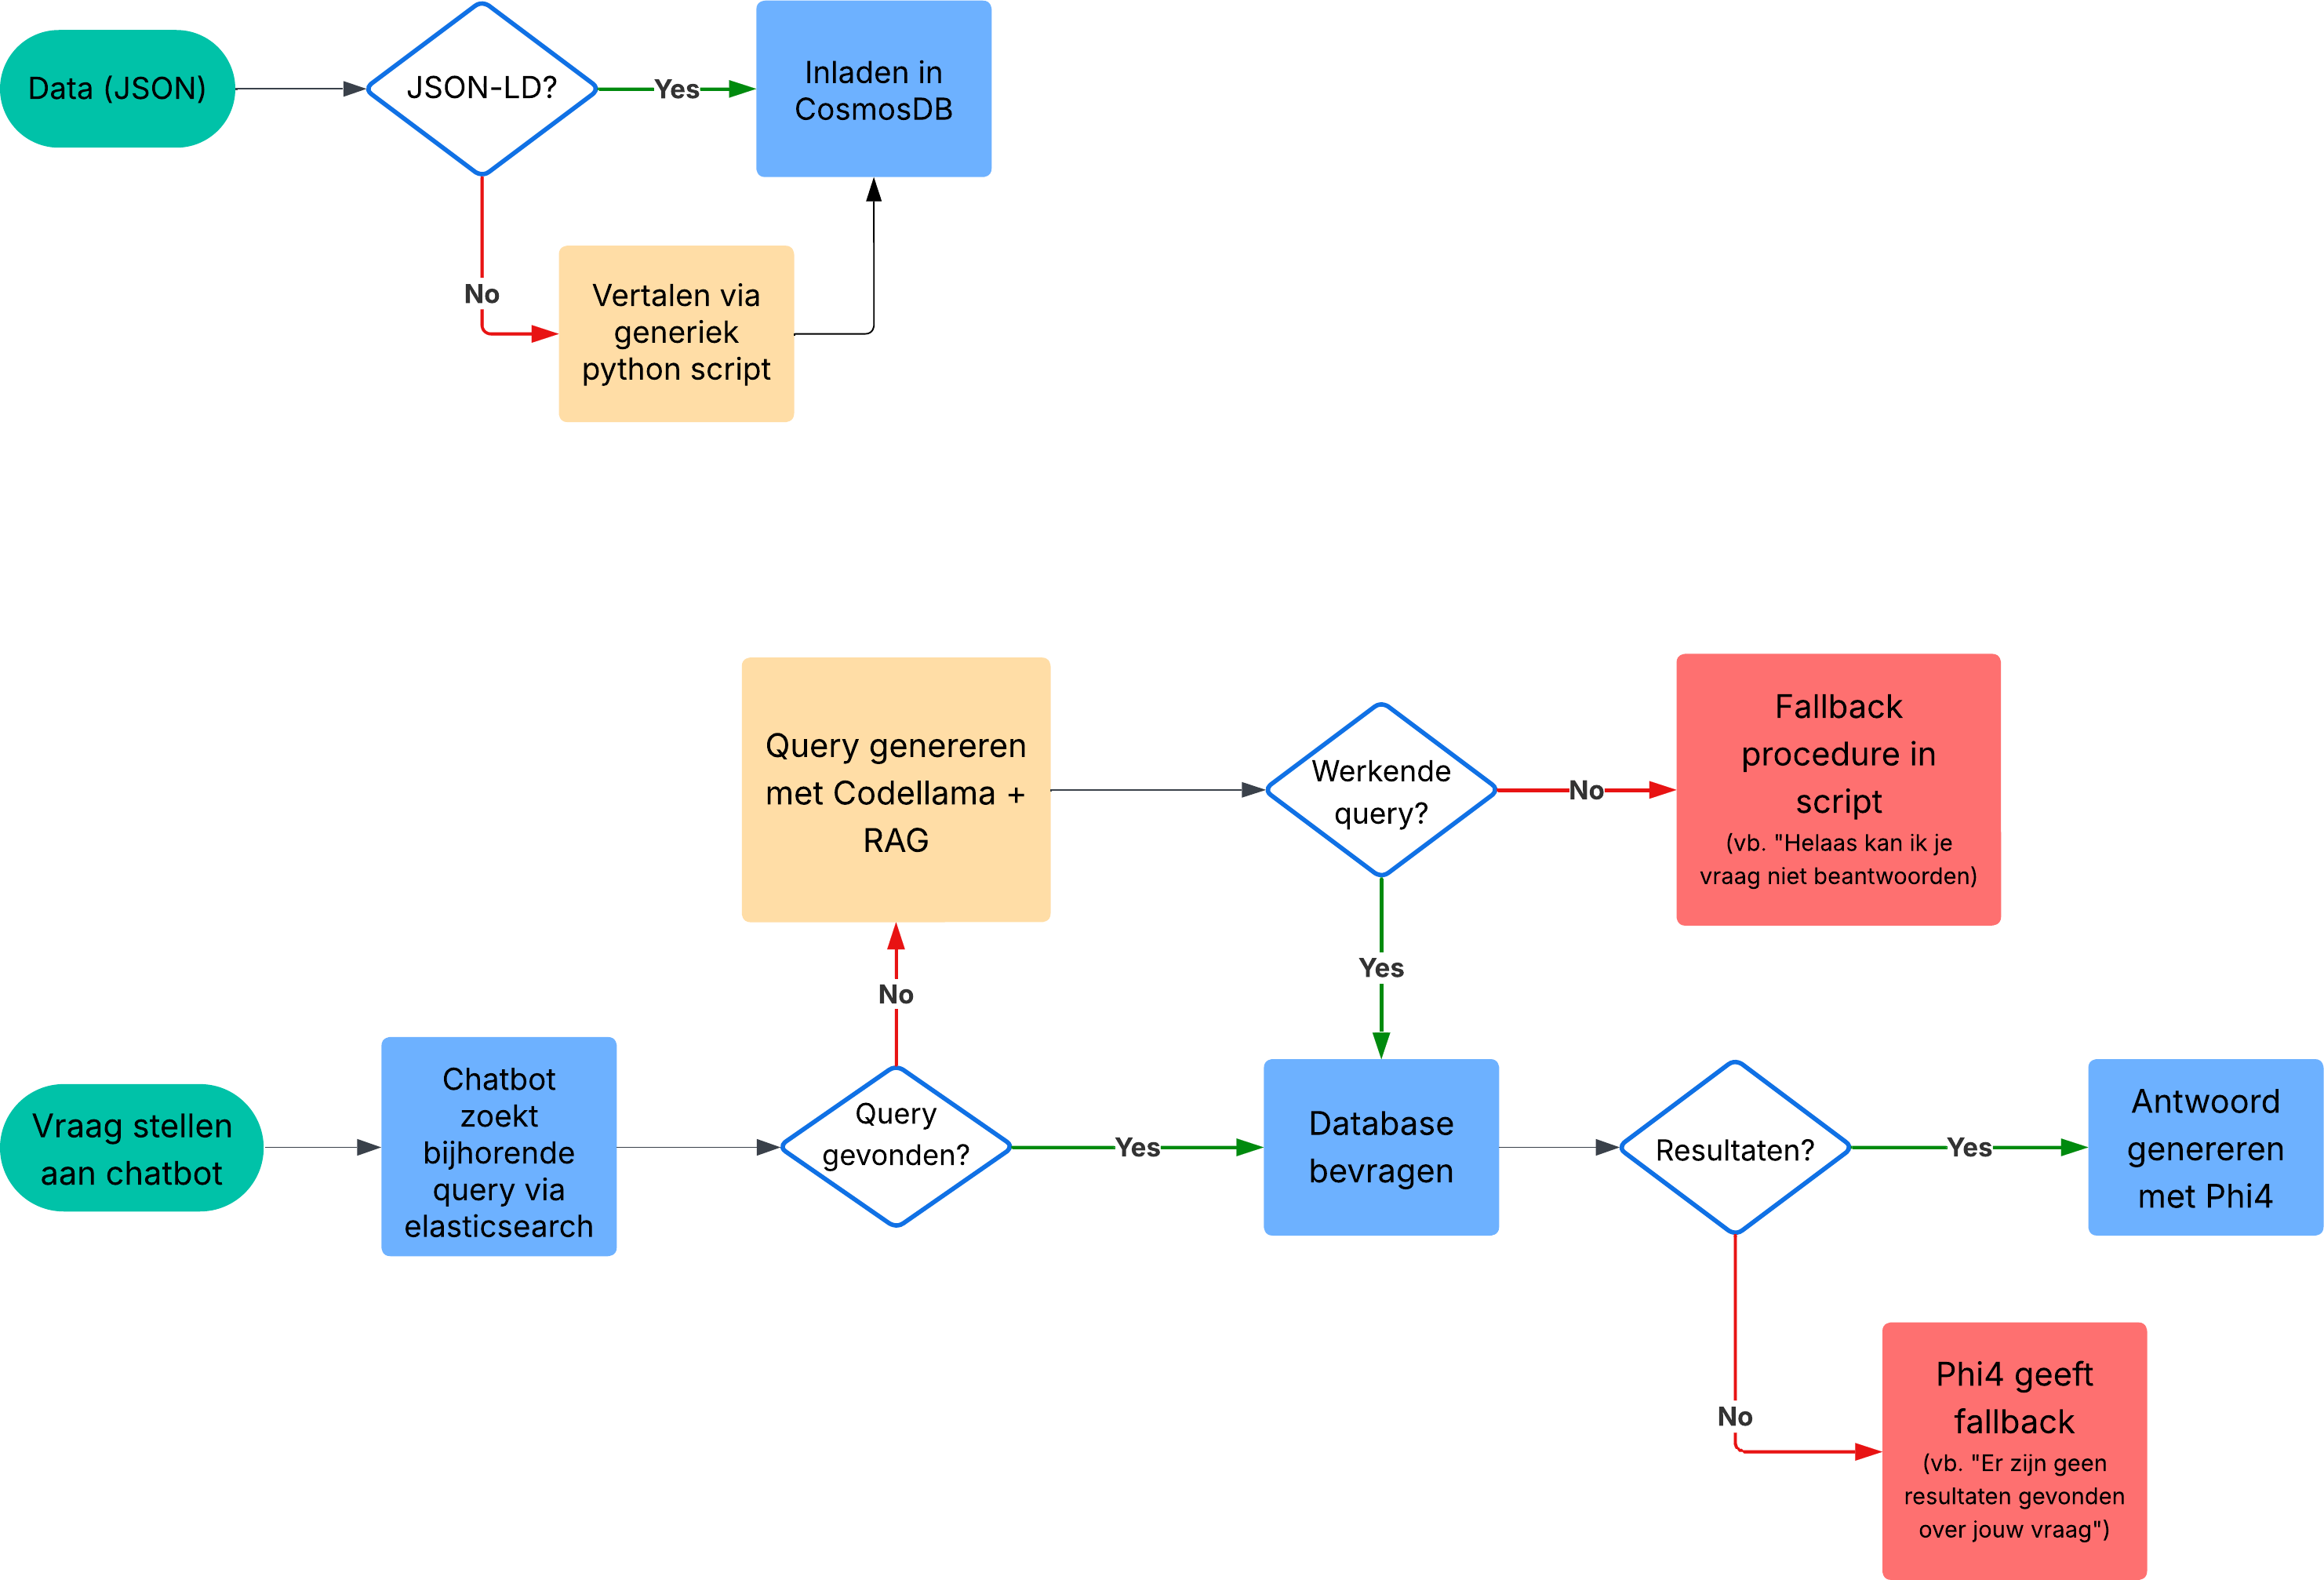
\includegraphics[width=0.8\textwidth]{./img/WorkflowThesis.png}
    \caption[Schema workflow]{\label{fig:workflow}Schema van workflow.}
\end{figure}

\subsection{Opzetten van een chatbot}
In het derde deel van deze bachelorproef wordt er een chatbot opgesteld die de data van het grafiekmodel kan bevragen en analyseren.
De input van dit model is een vraag die de gebruiker stelt, deze vraag wordt vertaald naar een Gremlin query die de data in CosmosDB zal bevragen.
Die kan dan op zijn beurt de relevante knopen en relaties vinden, die worden verwerkt en geformatteerd in leesbare tekst.
De chatbot is een iteratief proces, waarbij hij in de eerste iteratie de query maakt en in de tweede iteratie de resultaten teruggeeft aan de gebruiker.
Tijdens dit iteratief proces maken we gebruik van een Retrieval Augmented Generation (RAG) model dat de resultaten van de Gremlin query kan verwerken en formatteren naar een leesbare tekst.
Er zijn twee mogelijkheden om een query op te halen. De eerste methode maakt gebruik van Elasticsearch die in een docker container beschikbaar is. 
Daarbij gebruiken we een JSON bestand met voorbeeld vragen, die in een database geïndexeerd worden, om sneller en meer accuraat de juiste query te vinden.
De tweede methode maakt gebruik van de LLM indien er geen bijhorende query gevonden kan worden in de Elasticsearch.
Daarnaast valideren we de query die we terugkrijgen van het Large Language Model, zodat de query uitvoerbaar is in CosmosDB.\@

Daarnaast maken we ook gebruik van Docker om de verschillende componenten van de chatbot te beheren en te laten communiceren met elkaar.
Daardoor kunnen we de chatbot eenvoudig opzetten en beheren zonder dat we ons zorgen hoeven te maken over de onderliggende infrastructuur.
In figuur~\ref{fig:output} is een voorbeeld te zien van de output van de chatbot.
\begin{figure}[H]
    \centering
    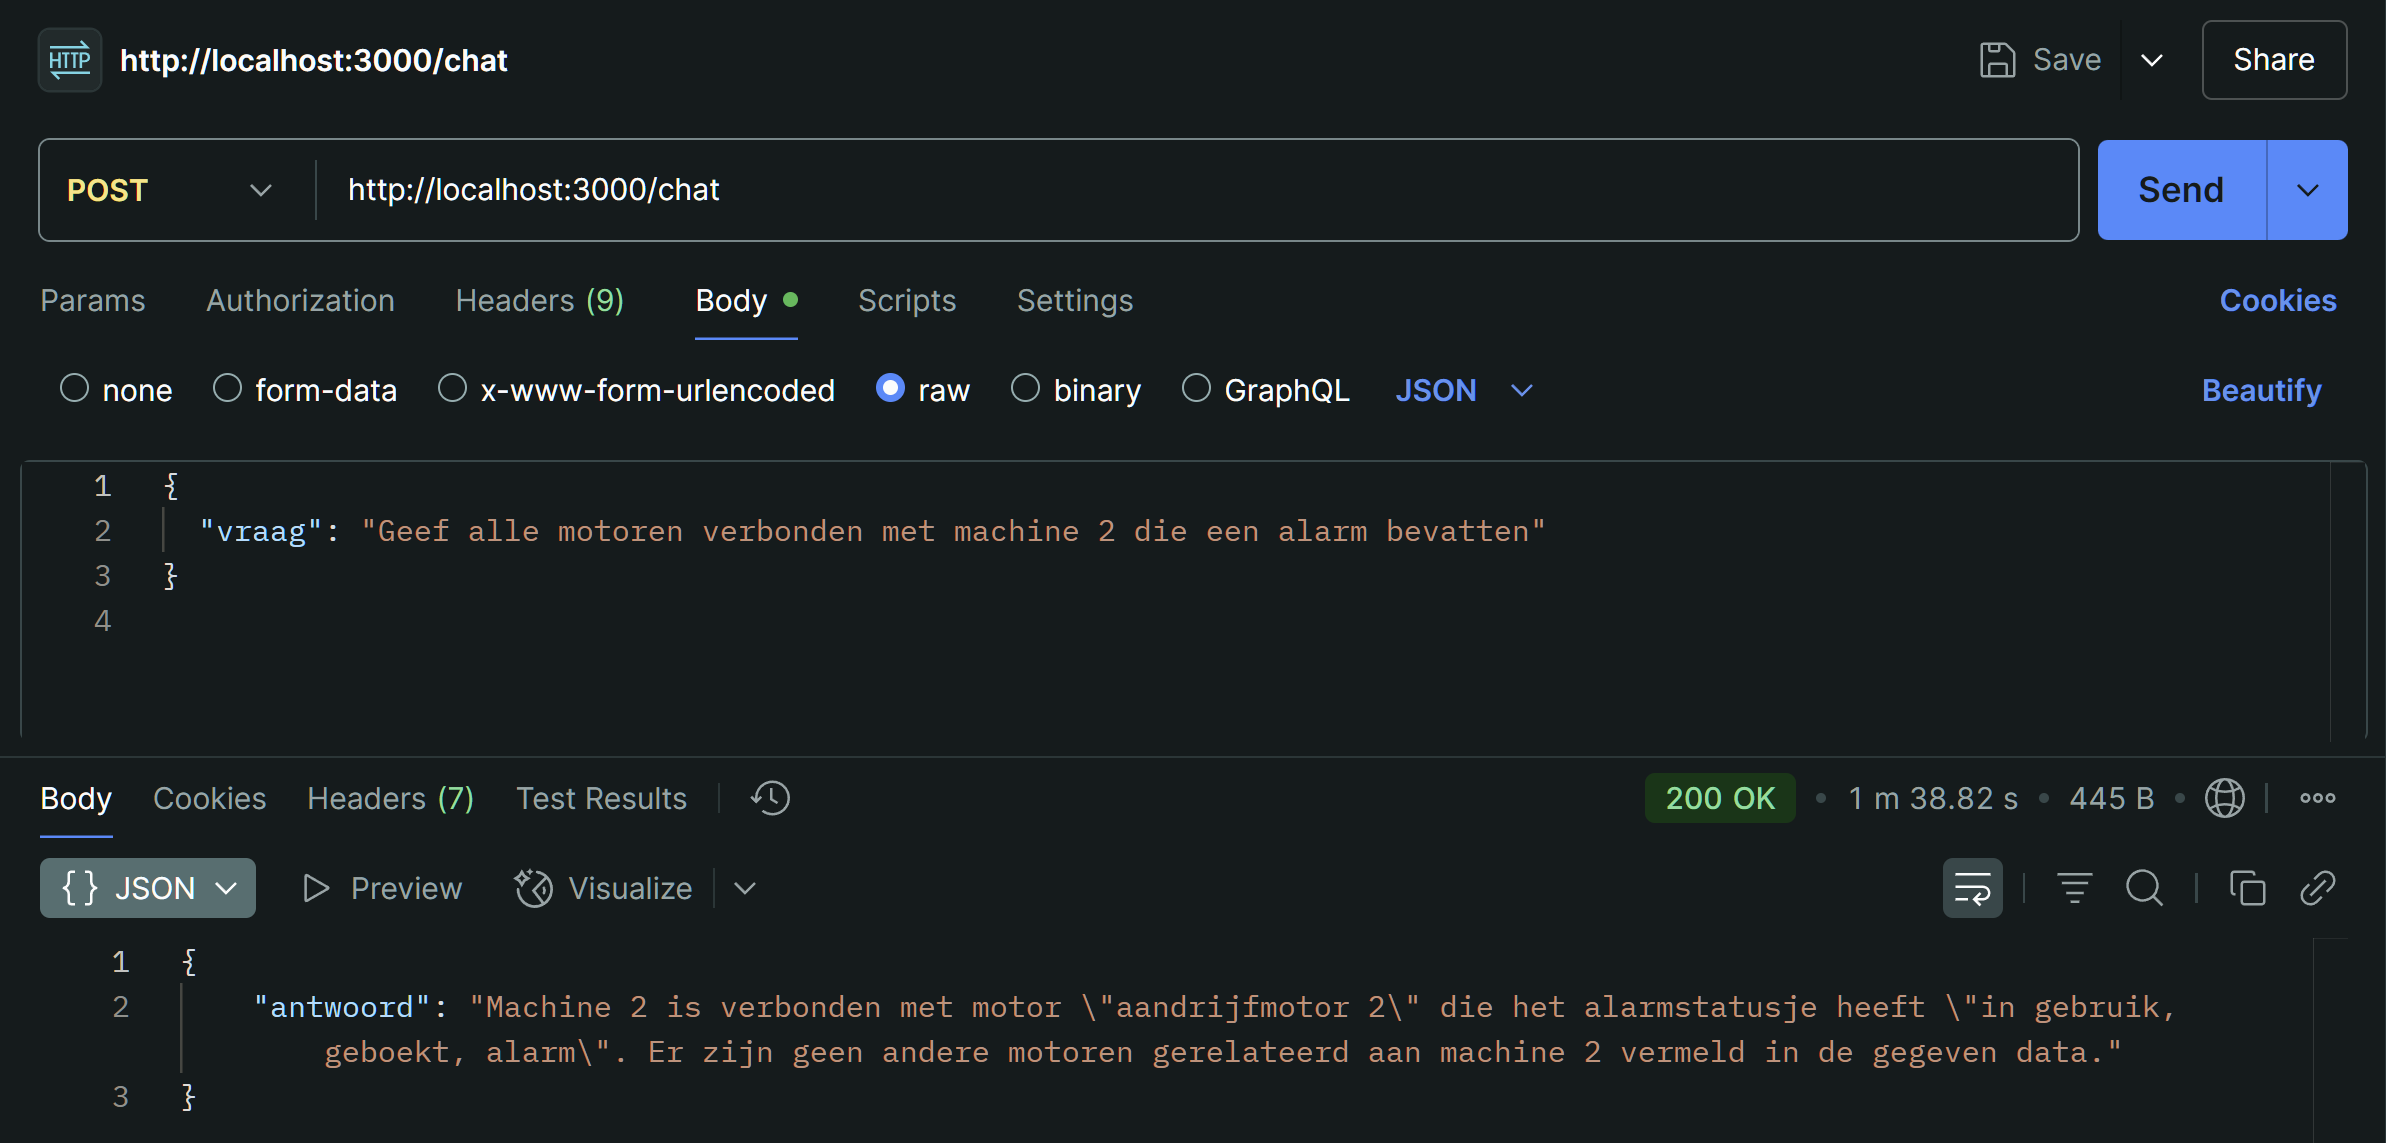
\includegraphics[width=0.8\textwidth]{./img/response.png}
    \caption[Output chatbot]{\label{fig:output}Voorbeeld van output op basis van CosmosDB.}
\end{figure}

\subsection{Structuur chatbot}
Voor onze chatbot maken we gebruik van CodeLlama voor het genereren van een Gremlin query en een Phi4 model voor het samenvatten van de data uit de database.
Deze modellen worden gebruikt via Ollama in een docker container zodat we een lokale versie gebruiken die niet verbonden is met het internet. Dit omdat we zeker willen zijn dat ons model geen data bijhoudt via het internet voor bijvoorbeeld het trainen van zijn eigen model.
Als voorbeeld van zo'n model die zichzelf trained hebben we OpenAI die een model heeft dat getraind is op een grote dataset, maar deze data wordt ook gebruikt om het model te verbeteren. 
Dit is niet de bedoeling voor ons model, want we willen zeker geen datalek veroorzaken.
Met de chatbot kunnen er een aantal vragen beantwoord worden die gerelateerd zijn aan het productieproces van ArcelorMittal Gent. Dit zijn vragen zoals: ``Welke fabrieken staan er in Gent'' of ``Geef alle kranen met een melding op de motor''.
Dit probleem lossen we op door het iteratief proces binnen onze chatbot waarbij we de vraag doorsturen naar de chatbot om het te beantwoorden.

\section{Resultaten}
De resultaten van dit eerste onderzoek zijn veelbelovend. Er is aangetoond dat het mogelijk is om een grafiekmodel op te zetten met behulp van CosmosDB en Gremlin API, en dat dit model kan worden gebruikt om data te visualiseren en analyseren.
Daarnaast is er een proof of concept ontwikkeld van een chatbot die in staat is om vragen te beantwoorden over het productieproces van ArcelorMittal Gent.
Het grootste probleem waar we nog tegen aanlopen is dat het CodeLlama model niet altijd de juiste Gremlin query genereert, waardoor we ze handmatig moeten toevoegen aan het JSON bestand voor Elasticsearch.
Dit kan opgelost worden door het model verder te trainen met LoRA, maar door beperkte tijd en resources is dit niet uitgevoerd in deze bachelorproef.

In volgende \href{https://youtu.be/D4-bSRYDLWM}{Demo video} is een korte demo te zien van de chatbot en hoe deze werkt met de data die we hebben opgezet in CosmosDB.\@
We zien dat de chatbot in het begin even de tijd nodig heeft om de vraag te beantwoorden, dit komt doordat Ollama stand by staat, maar het model nog niet geladen heeft.
Pas als de vraag wordt gesteld, wordt het model geladen en kan de chatbot de vraag beantwoorden. 
Bij de tweede vraag gaat dit veel sneller omdat het model al geladen is en de chatbot de vraag direct kan beantwoorden.



\subsection{Voordelen}
De voordelen van het gebruik van een tijdelijk grafiekmodel zijn onder andere:
\begin{itemize}
    \item Het is mogelijk om data te visualiseren en analyseren door de relaties tussen de verschillende producten en processen.
    \item Het is mogelijk om snel vragen van gebruikers te beantwoorden over het productieproces van ArcelorMittal Gent.
    \item Verhoogde traceerbaarheid van productieprocessen, waardoor het eenvoudiger wordt om problemen te identificeren en op te lossen.
    \item Het is mogelijk om de chatbot eenvoudig op te zetten en te beheren zonder dat we ons zorgen hoeven te maken over de onderliggende infrastructuur.
    \item Door gebruik te maken van Elasticsearch kunnen we sneller een antwoord geven op meest gestelde vragen, waardoor de chatbot sneller en efficiënter wordt.
\end{itemize}

\subsection{Voordelen}
De nadelen of problemen die ondervonden zijn bij de huidige werkwijze zijn onder andere:
\begin{itemize}
    \item Het CodeLlama model genereert niet altijd de juiste Gremlin query, waardoor we ze handmatig moeten toevoegen aan het JSON bestand voor Elasticsearch.
    \item De snelheid van de chatbot is afhankelijk van Ollama die een antwoord of query moet genereren, waardoor het soms langer duurt om een antwoord te krijgen indien de query niet in Elasticsearch aanwezig is.
\end{itemize}

\section{Toekomstvisie}
Om de chatbot verder uit te breiden en te verbeteren zijn er verschillende zaken die kunnen worden aangepakt.
Eerst en vooral kan er gekeken worden naar het finetunen van het CodeLlama model met LoRA zoals besproken in~\ref{sec:LORA} om de kwaliteit van de gegenereerde Gremlin queries te verbeteren.
Daarnaast kunnen er nog meer performantie optimalisaties worden doorgevoerd om de snelheid van de chatbot te verhogen.
Ook kunnen er eventueel rechten worden toegevoegd zodat bepaalde gebruikersgroepen enkel bepaalde vragen kunnen stellen of antwoorden kunnen krijgen.
Hiernaast kunnen deze rechten ook gebruikt worden om de DELETE, ADD en UPDATE acties toe te voegen om de chatbot multifunctioneel te maken.


%% TODO: In dit hoofstuk geef je een korte toelichting over hoe je te werk bent
%% gegaan. Verdeel je onderzoek in grote fasen, en licht in elke fase toe wat
%% de doelstelling was, welke deliverables daar uit gekomen zijn, en welke
%% onderzoeksmethoden je daarbij toegepast hebt. Verantwoord waarom je
%% op deze manier te werk gegaan bent.
%% 
%% Voorbeelden van zulke fasen zijn: literatuurstudie, opstellen van een
%% requirements-analyse, opstellen long-list (bij vergelijkende studie),
%% selectie van geschikte tools (bij vergelijkende studie, "short-list"),
%% opzetten testopstelling/PoC, uitvoeren testen en verzamelen
%% van resultaten, analyse van resultaten, ...
%%
%% !!!!! LET OP !!!!!
%%
%% Het is uitdrukkelijk NIET de bedoeling dat je het grootste deel van de corpus
%% van je bachelorproef in dit hoofstuk verwerkt! Dit hoofdstuk is eerder een
%% kort overzicht van je plan van aanpak.
%%
%% Maak voor elke fase (behalve het literatuuronderzoek) een NIEUW HOOFDSTUK aan
%% en geef het een gepaste titel.



